\documentclass[11pt,a4paper]{article}
\usepackage[margin=19mm,top=24mm,bottom=22mm,headheight=15pt]{geometry}
\usepackage{fontspec,amsmath,amssymb,xcolor,fancyhdr,tabularx,tikz}
\setmainfont{texgyreheros-regular.otf}[BoldFont=texgyreheros-bold.otf,ItalicFont=texgyreheros-italic.otf]
\setsansfont{texgyreheros-regular.otf}[BoldFont=texgyreheros-bold.otf]
\setmonofont{texgyrecursor-regular.otf}
\definecolor{ink}{HTML}{18324E}
\definecolor{muted}{HTML}{526176}
\definecolor{line}{HTML}{DCE3EB}
\color{ink}
\setlength{\parindent}{0pt}
\setlength{\parskip}{7pt}
\pagestyle{fancy}\fancyhf{}
\fancyhead[L]{\small\textbf{EAZYGRADES}}
\fancyhead[R]{\small COMP 352 / CORE}
\fancyfoot[L]{\scriptsize\shortstack[l]{\copyright\ 2026 EazyGrades. For personal study use only.\\Redistribution, resale, or sharing is not permitted.}}
\fancyfoot[R]{\small\thepage}
\renewcommand{\headrulewidth}{0.6pt}
\renewcommand{\footrulewidth}{0.3pt}
\newcommand{\pagetitle}[2]{\textcolor{muted}{\small\MakeUppercase{#1}}\par\vspace{4pt}{\LARGE\bfseries #2}\par\vspace{10pt}}
\newcommand{\qtitle}[1]{\par\noindent{\large\bfseries #1}\par\vspace{3pt}}
\newcommand{\worklines}{\par\vspace{3pt}{\color{line}\hrule}\vspace{17pt}{\color{line}\hrule}\vspace{17pt}{\color{line}\hrule}\vspace{13pt}}
\begin{document}
\pagetitle{Outline-based practice}{Core Exam Practice}
{\Large\bfseries COMP 352}\par
{\large Data Structures and Algorithms}\par\vspace{14pt}
8 multiple-choice questions\quad\textbullet\quad 6 true/false questions\par
10 long answer questions\quad\textbullet\quad Answer key included\par\vspace{16pt}
\qtitle{Before you begin}
Show your reasoning and use additional paper as needed. Try the questions before checking the solutions.

\textbf{120 practice marks.} Multiple choice: 1 mark each. True/false: 1 mark for the answer and 1 for the explanation. Long answer questions: 10 marks each. No negative marking in this practice set.\par
\vspace{16pt}
\qtitle{Topics}
Algorithm analysis and recursion; arrays, stacks and queues; linked lists; trees and heaps; hashing and sorting; graphs and data-structure design.
\vfill
{\small\color{muted}Based on the supplied COMP 352 Winter 2025 course outline. Selected topics only; not a complete syllabus review or a prediction of your exam.\par
AI-generated practice for study and revision only. Not official course material. EazyGrades is not affiliated with Concordia University or any school. No academic result is guaranteed.}
\newpage
\pagetitle{Section A / 8 marks}{Multiple choice}
Choose one answer for each question.\par
\begin{minipage}{\linewidth}
\textbf{M1.} Which is a tight bound for $5n^{2}+3n+8$?\par
\renewcommand{\arraystretch}{1.4}\begin{tabularx}{\linewidth}{@{}X X@{}}
\textbf{A.}\enspace $O(n)$ & \textbf{B.}\enspace $\Theta(n^2)$ \\
\textbf{C.}\enspace $\Theta(n^3)$ & \textbf{D.}\enspace $\Theta(\log\,n)$
\end{tabularx}\end{minipage}\par\vspace{7pt}
\begin{minipage}{\linewidth}
\textbf{M2.} Which structure naturally implements recursive-call bookkeeping?\par
\renewcommand{\arraystretch}{1.4}\begin{tabularx}{\linewidth}{@{}X X@{}}
\textbf{A.}\enspace queue & \textbf{B.}\enspace hash table \\
\textbf{C.}\enspace stack & \textbf{D.}\enspace sorted array
\end{tabularx}\end{minipage}\par\vspace{7pt}
\begin{minipage}{\linewidth}
\textbf{M3.} Worst-case access to index $i$ in a singly linked list of $n$ nodes?\par
\renewcommand{\arraystretch}{1.4}\begin{tabularx}{\linewidth}{@{}X X@{}}
\textbf{A.}\enspace $\Theta(1)$ & \textbf{B.}\enspace $\Theta(\log\,n)$ \\
\textbf{C.}\enspace $\Theta(n)$ & \textbf{D.}\enspace $\Theta(n\,\log\,n)$
\end{tabularx}\end{minipage}\par\vspace{7pt}
\begin{minipage}{\linewidth}
\textbf{M4.} In a zero-based binary heap, the left child of index $i$ is at:\par
\renewcommand{\arraystretch}{1.4}\begin{tabularx}{\linewidth}{@{}X X@{}}
\textbf{A.}\enspace $2i$ & \textbf{B.}\enspace $2i+1$ \\
\textbf{C.}\enspace $\frac{i}{2}$ & \textbf{D.}\enspace $2i+2$
\end{tabularx}\end{minipage}\par\vspace{7pt}
\begin{minipage}{\linewidth}
\textbf{M5.} Which traversal of a BST with distinct keys produces sorted order?\par
\renewcommand{\arraystretch}{1.4}\begin{tabularx}{\linewidth}{@{}X X@{}}
\textbf{A.}\enspace preorder & \textbf{B.}\enspace postorder \\
\textbf{C.}\enspace level-order & \textbf{D.}\enspace inorder
\end{tabularx}\end{minipage}\par\vspace{7pt}
\begin{minipage}{\linewidth}
\textbf{M6.} A hash table uses $h(k)=k\bmod 7$. Which pair of keys collides?\par
\renewcommand{\arraystretch}{1.4}\begin{tabularx}{\linewidth}{@{}X X@{}}
\textbf{A.}\enspace 10 and 17 & \textbf{B.}\enspace 10 and 18 \\
\textbf{C.}\enspace 5 and 13 & \textbf{D.}\enspace 7 and 15
\end{tabularx}\end{minipage}\par\vspace{7pt}
\begin{minipage}{\linewidth}
\textbf{M7.} Typical array mergesort worst-case time is:\par
\renewcommand{\arraystretch}{1.4}\begin{tabularx}{\linewidth}{@{}X X@{}}
\textbf{A.}\enspace $\Theta(n)$ & \textbf{B.}\enspace $\Theta(n^2)$ \\
\textbf{C.}\enspace $\Theta(n\,\log\,n)$ & \textbf{D.}\enspace $\Theta(2^n)$
\end{tabularx}\end{minipage}\par\vspace{7pt}
\begin{minipage}{\linewidth}
\textbf{M8.} Two unequal keys hashing to one index is called:\par
\renewcommand{\arraystretch}{1.4}\begin{tabularx}{\linewidth}{@{}X X@{}}
\textbf{A.}\enspace recursion & \textbf{B.}\enspace collision \\
\textbf{C.}\enspace traversal & \textbf{D.}\enspace rotation
\end{tabularx}\end{minipage}\par\vspace{7pt}
\newpage\pagetitle{Section B / 12 marks}{True or false}
Give a brief justification for each answer.\par
\textbf{T1.} Every binary search tree has logarithmic height.\par\worklines
\textbf{T2.} An array-based stack can have amortized $O(1)$ push with occasional linear work.\par\worklines
\textbf{T3.} A min-heap array must be globally sorted.\par\worklines
\textbf{T4.} Binary search works correctly on any unsorted array.\par\worklines
\textbf{T5.} A hash-table lookup is always worst-case $O(1)$.\par\worklines
\textbf{T6.} BFS gives minimum-edge-count paths from its source in an unweighted graph.\par\worklines
\newpage\pagetitle{Section C / 20 marks}{Analysis and recursion}
\qtitle{Q1. Algorithm analysis / 10 marks}
(a) Let $n$ be a positive power of two. For the pseudocode below, give the exact number of calls to $\operatorname{work}()$ and a tight asymptotic bound. Each call takes constant time. (4 marks)\par
\begin{quote}\small
$i\gets 1$\\
\textbf{while} $i\leq n$:\\
\hspace*{1em}\textbf{for} $j\gets 1$ \textbf{to} $i$:\\
\hspace*{2em}$\operatorname{work}()$\\
\hspace*{1em}$i\gets 2i$
\end{quote}
(b) Order these functions by increasing asymptotic growth: $n\log_2 n$, $2^n$, $\log_2 n$, $n^2$, $n$. (3 marks)\par
(c) Is $3n+7$ in $O(n^2)$? Is it in $\Theta(n^2)$? Explain the distinction. (3 marks)\par
\worklines
\qtitle{Q2. Recursion and correctness / 10 marks}
(a) For powers of two, $T(1)=1$ and $T(n)=2T\!\left(\frac{n}{2}\right)+n$. Give the exact solution and explain the work at each recursion level. (4 marks)\par
(b) Recursive binary search uses $\mathit{mid}=\left\lfloor\frac{\mathit{lo}+\mathit{hi}}{2}\right\rfloor$. On a sorted array, it recurses into $[\mathit{lo},\mathit{mid}-1]$ or $[\mathit{mid}+1,\mathit{hi}]$. State the empty-range base case and explain termination. (3 marks)\par
(c) State binary search worst-case time and recursive auxiliary space. How does an iterative version change the space bound? (3 marks)\par
\worklines
\newpage\pagetitle{Section C / 20 marks}{Linear data structures}
\qtitle{Q3. Arrays, stacks and queues / 10 marks}
(a) A circular queue has capacity 5, $\mathit{front}=3$ and $\mathit{size}=3$. Its logical contents are $A$, $B$, $C$ in that order. Show physical indices. Dequeue once, then enqueue $D$ and $E$; give final $\mathit{front}$, $\mathit{size}$ and array slots. (4 marks)\par
(b) Starting empty, execute $\operatorname{push}(4)$, $\operatorname{push}(7)$, $\operatorname{pop}()$, $\operatorname{push}(2)$, $\operatorname{push}(9)$, $\operatorname{pop}()$. List returned values and final stack, bottom to top. (3 marks)\par
(c) An array doubles capacity when full. Explain why append is amortized $O(1)$ even though one append can take $\Theta(n)$. (3 marks)\par
\worklines
\qtitle{Q4. Linked lists and implementation / 10 marks}
(a) Write Java-like pseudocode to reverse a singly linked list in place. Preserve every node, return the new $\mathit{head}$, and handle an empty list. (5 marks)\par
(b) Give tight time and auxiliary-space bounds for your reversal. (2 marks)\par
(c) With $\mathit{head}$ and $\mathit{tail}$ pointers, compare removing the last node of a singly linked list and a doubly linked list. Explain. (3 marks)\par
\worklines
\newpage\pagetitle{Section C / 20 marks}{Trees and priority queues}
\qtitle{Q5. Trees, traversals and search / 10 marks}
(a) Insert 7, 3, 9, 1, 5 into an empty binary search tree. Draw the tree, then give inorder and preorder traversals. (4 marks)\par
(b) Delete 7 using its inorder successor as the replacement. Draw the resulting tree and state the successor. (3 marks)\par
(c) Define height as the number of edges on the longest root-to-leaf path. Give the original height and search cost in terms of height; compare balanced and degenerate trees. (3 marks)\par
\worklines
\qtitle{Q6. Priority queues and heaps / 10 marks}
(a) Insert 6, 2, 9, 1, 5 into an empty binary min-heap. Show the level-order array after each insertion. Use zero-based indexing. (4 marks)\par
(b) Perform removeMin on the final heap. Show the replacement and down-heap swaps, then the final array. (3 marks)\par
(c) Draw the binary min-heap as a tree after the removeMin operation in part (b). Label every node with its key and briefly explain why the result satisfies the min-heap property. (3 marks)\par
\vspace{3pt}{\color{line}\fbox{\parbox[t][85pt][t]{0.95\linewidth}{\small\color{muted}Tree drawing}}}\par
\newpage\pagetitle{Section C / 20 marks}{Hashing and sorting}
\qtitle{Q7. Maps and hash tables / 10 marks}
(a) Insert keys 10, 17, 24, 5 into a table of size 7 using $h(k)=k\bmod 7$ and linear probing. Show occupied indices and the load factor. (4 marks)\par
(b) Delete key 17. Why should its slot be marked with a tombstone rather than made never-used? Trace a search for 24. (3 marks)\par
(c) Contrast expected lookup under well-distributed hashes and controlled load with worst-case lookup. What can cause the worst case? (3 marks)\par
\worklines
\qtitle{Q8. Sorting and algorithm choice / 10 marks}
(a) Trace insertion sort on $[4,1,3,2]$, giving the whole array after each outer-loop pass. State worst-case time and auxiliary space. (4 marks)\par
(b) Merge sorted runs $[2,6,8]$ and $[1,3,7]$. Give the result and number of key comparisons; stop comparing when one run is exhausted. (3 marks)\par
(c) Which is preferable for a nearly sorted small array: insertion sort or a typical mergesort implementation? Explain, and define stability for equal-key records. (3 marks)\par
\worklines
\newpage\pagetitle{Section C / 20 marks}{Graphs and design}
\qtitle{Q9. Graph representation and traversal / 10 marks}
Use an undirected graph with vertices $A,B,C,D,E,F$ and edges $AB,AC,BD,CD,DE$. Visit neighbors alphabetically. (a) Give adjacency lists and BFS discovery order from $A$, including distances and parents. (5 marks)\par
(b) Give recursive DFS discovery order from $A$. Is $F$ reachable? (2 marks)\par
(c) Give a shortest A-to-E path. Explain why BFS finds shortest paths in unweighted graphs, and state its adjacency-list time bound. (3 marks)\par
\worklines
\qtitle{Q10. Choosing structures and designing operations / 10 marks}
A task scheduler stores unique task IDs with integer priorities. Smaller numbers run first; tied priorities may run in either order. It supports add, lookup by ID, and remove-next. (a) Propose a combination of data structures and explain what each stores. (4 marks)\par
(b) State the expected cost of each operation and describe how you keep the structures consistent when removing the next task. (3 marks)\par
(c) If priority changes by ID must take $O(\log\,n)$ expected time, what extra information must you maintain? Explain how updates preserve it. (3 marks)\par
\worklines
\newpage\pagetitle{Solutions / Sections $A$ and B}{Concept-check answers}
\qtitle{Multiple choice}
\textbf{M1.} B: the quadratic term dominates.\par
\textbf{M2.} C: the most recent unfinished call resumes first.\par
\textbf{M3.} C: reaching a late position requires following links.\par
\textbf{M4.} B: left child is $2i+1$; right child is $2i+2$.\par
\textbf{M5.} D: left subtree, node, right subtree.\par
\textbf{M6.} A: $10\bmod 7=3$ and $17\bmod 7=3$, so both keys hash to index 3.\par
\textbf{M7.} C: linear merging across logarithmically many levels.\par
\textbf{M8.} B: collisions require a resolution strategy.\par
\vspace{8pt}\qtitle{True or false}
\textbf{T1.} False. Sorted insertions into an unbalanced BST can produce height $n-1$.\par
\textbf{T2.} True. Geometric capacity growth spreads total copying over many pushes.\par
\textbf{T3.} False. Parent-child order does not order siblings or unrelated subtrees.\par
\textbf{T4.} False. Its half-discarding argument depends on sorted order.\par
\textbf{T5.} False. Collisions can force a linear probe sequence or long bucket.\par
\textbf{T6.} True. Vertices are first discovered in nondecreasing distance layers.\par
\newpage\pagetitle{Solutions / Section C}{Worked solutions 1--2}
\qtitle{Q1. Algorithm analysis}
(a) The work is $1+2+\cdots+n=2n-1$, hence $\Theta(n)$. There are $\log_2 n+1$ outer iterations, but their costs are not all $n$. Award 2 marks for the sum, 1 for its value, 1 for the bound.\par
(b) $\log_2 n$, $n$, $n\log_2 n$, $n^2$, $2^n$. This is an eventual-growth comparison, not a claim about every small $n$. Award 3 marks for the full ordering; 2 for one adjacent inversion.\par
(c) Yes to $O(n^2)$: for $n\geq 1$, $3n+7\leq 10n^2$. No to $\Theta(n^2)$, since $\frac{3n+7}{n^2}$ tends to 0. Its tight growth is $\Theta(n)$. Award one mark for each conclusion and one for reasoning.\par
\vspace{12pt}
\qtitle{Q2. Recursion and correctness}
(a) There are $\log_2 n$ internal levels, each doing $n$ nonrecursive work. The $n$ leaves contribute $n$, so $T(n)=n\log_2 n+n=\Theta(n\log n)$. Award 2 marks for level work/depth, 1 for leaves, 1 for the result.\par
(b) If $\mathit{lo}>\mathit{hi}$, return not found. Otherwise either the midpoint matches or the next interval is strictly smaller, because $\mathit{mid}$ is excluded. A nonnegative interval size cannot decrease forever. Award one mark each for base case, shrinking range and termination argument.\par
(c) Worst-case time is $\Theta(\log\,n)$, with $\Theta(\log\,n)$ recursive stack space. Iteration uses $\Theta(1)$ auxiliary space. Award one mark each. Assume constant-time array access.\par
\vspace{12pt}
\newpage\pagetitle{Solutions / Section C}{Worked solutions 3--4}
\qtitle{Q3. Arrays, stacks and queues}
(a) Initially $A$ is at 3, $B$ at 4, $C$ at 0. Removing $A$ gives $\mathit{front}=4$, $\mathit{size}=2$. $D$ goes to $(4+2)\bmod 5=1$; $E$ goes to $(4+3)\bmod 5=2$. Final $\mathit{front}=4$, $\mathit{size}=4$, slots $0,\ldots,4$ contain $[C,D,E,\text{unused},B]$. Award one mark per stage; stale removed data in slot 3 is acceptable if labelled inactive.\par
(b) The pops return 7 and 9. The final stack is $[4, 2]$ bottom to top. Award 1 mark for each pop and 1 for the stack.\par
(c) With initial capacity 1, resizing copies $1+2+4+\cdots$ items, totaling less than $2n$ over $n$ appends. Including $n$ new writes gives $O(n)$ total work and $O(1)$ amortized cost. A resizing append copies all current items. Award one mark for the series, one for total/amortized cost, one for the single-operation caveat.\par
\vspace{12pt}
\qtitle{Q4. Linked lists and implementation}
(a) Initialize $\mathit{prev}=\mathrm{null}$ and $\mathit{curr}=\mathit{head}$. While $\mathit{curr}\ne\mathrm{null}$: save $\mathit{next}=\mathit{curr}.\mathit{next}$; set $\mathit{curr}.\mathit{next}=\mathit{prev}$; set $\mathit{prev}=\mathit{curr}$; set $\mathit{curr}=\mathit{next}$. Return $\mathit{prev}$. Saving $\mathit{next}$ before changing the link prevents losing the unprocessed suffix. Empty input returns $\mathrm{null}$. Award 1 mark each for initialization, saved $\mathit{next}$, link reversal, pointer progress, and return/empty handling.\par
(b) Each node is processed once: $\Theta(n)$ time and $\Theta(1)$ auxiliary space. Award one mark each.\par
(c) A singly linked list needs $\Theta(n)$ worst-case time to locate the predecessor of $\mathit{tail}$; $\mathit{tail}$ alone cannot identify it. A doubly linked list uses $\mathit{tail}.\mathit{prev}$ in $\Theta(1)$ time. Handle the singleton case by clearing $\mathit{head}$ and $\mathit{tail}$, otherwise clear the new $\mathit{tail}.\mathit{next}$. Award one mark per complexity and one for explanation/boundaries.\par
\vspace{12pt}
\newpage\pagetitle{Solutions / Section C}{Worked solutions 5--6}
\qtitle{Q5. Trees, traversals and search}
(a) Root 7 has left child 3 and right child 9; node 3 has children 1 and 5. Inorder: 1, 3, 5, 7, 9. Preorder: 7, 3, 1, 5, 9. Award 2 marks for the tree and 1 per traversal.\par
(b) The minimum node in the right subtree is 9, the successor. Replace 7 with 9 and remove its original node. Root 9 now has only left child 3, whose children remain 1 and 5. Award one mark for successor and two for the resulting structure.\par
(c) Original height $h=2$. Worst-case search is $O(h+1)$, commonly written $O(h)$ for positive heights. Balanced trees give $O(\log\,n)$; a degenerate tree gives $O(n)$. Award one mark for height, one for height-based work and one for the comparison.\par
\vspace{12pt}
\qtitle{Q6. Priority queues and heaps}
(a) Arrays: $[6]$; $[2,6]$; $[2,6,9]$; $[1,2,9,6]$; $[1,2,9,6,5]$. The parent of index $i>0$ is $\left\lfloor\frac{i-1}{2}\right\rfloor$. Up-heap swaps restore $\mathit{parent}\leq\mathit{child}$. Award 1 mark for each of the final four arrays.\par
(b) Return 1. Move the last key 5 to root: $[5,2,9,6]$. Swap with smaller child 2, yielding $[2,5,9,6]$. Now $5\leq 6$, so stop. Award one mark each for returned/replacement values, chosen swap and final heap.\par
(c) The resulting tree has root 2, left child 5 and right child 9; node 5 has left child 6. Every parent is no larger than its children: $2\leq 5$, $2\leq 9$ and $5\leq 6$. The shape is complete, with the last level filled from left to right. Award 2 marks for the correct labelled tree and 1 for the heap-property explanation.\par
\begin{center}
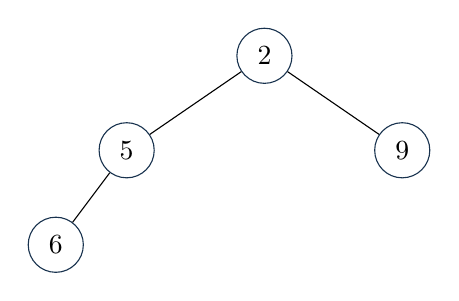
\begin{tikzpicture}[level distance=12mm,level 1/.style={sibling distance=35mm},level 2/.style={sibling distance=18mm},every node/.style={circle,draw=ink,minimum size=7mm}]
\node {2} child {node {5} child {node {6}} child[missing]} child {node {9}};
\end{tikzpicture}\end{center}
\vspace{12pt}
\newpage\pagetitle{Solutions / Section C}{Worked solutions 7--8}
\qtitle{Q7. Maps and hash tables}
(a) 10 goes to 3, 17 probes to 4, 24 probes to 5, and 5 probes to 6. Load factor is $\frac{4}{7}$. Award 3 marks for correct placements and 1 for load factor.\par
(b) Index 4 becomes a tombstone. Searching for 24 begins at 3, skips 10, passes the tombstone at 4, and finds 24 at 5. A never-used slot would incorrectly terminate the search at 4. Award one mark for deletion marker, trace and explanation.\par
(c) Expected lookup is $O(1)$ under suitable hashing and a load factor bounded away from 1. Worst-case lookup is $O(n)$ for a table of size $\Theta(n)$, because many collisions can form a long probe cluster. Award one mark per bound and one for cause/assumptions.\par
\vspace{12pt}
\qtitle{Q8. Sorting and algorithm choice}
(a) Passes: $[1,4,3,2]$, $[1,3,4,2]$, $[1,2,3,4]$. Worst-case time is $\Theta(n^2)$, auxiliary space $\Theta(1)$. Award 2 marks for the passes and 1 per bound.\par
(b) Result: $[1,2,3,6,7,8]$. Compare $(2,1)$, $(2,3)$, $(6,3)$, $(6,7)$, $(8,7)$: five comparisons, then append 8. Award 1 mark for output and 2 for count/trace.\par
(c) Insertion sort is often preferable because overhead is small and only a few shifts are needed; this is a practical choice, not a universal performance guarantee. A stable sort preserves original relative order among equal-key records. Insertion sort is stable if it shifts only strictly larger keys. Award one mark for choice, reason and definition.\par
\vspace{12pt}
\newpage\pagetitle{Solutions / Section C}{Worked solutions 9--10}
\qtitle{Q9. Graph representation and traversal}
(a) Lists: $A: B,C$; $B: A,D$; $C: A,D$; $D: B,C,E$; $E: D$; $F: \varnothing$. BFS discovers $A,B,C,D,E$. Distances are $0,1,1,2,3$, respectively; $F$ is unreachable. Parents: $B\leftarrow A$, $C\leftarrow A$, $D\leftarrow B$, $E\leftarrow D$. Award 2 marks for lists, 1 for order, 1 for distances and 1 for parents.\par
(b) DFS discovers $A,B,D,C,E$. $F$ is not reachable from $A$. Award one mark each. This is recursive DFS; returning from $C$ to $D$ precedes discovering $E$.\par
(c) $A\to B\to D\to E$ has length 3 ($A\to C\to D\to E$ is also shortest). A FIFO queue processes vertices in increasing distance layers, so first discovery supplies a shortest path in edge count. The standard full-graph bound is $O(V+E)$, including initialization. Award one mark each for path, reasoning and bound.\par
\vspace{12pt}
\qtitle{Q10. Choosing structures and designing operations}
(a) Use a binary min-heap of task records for priority order and a hash map from ID to the task record (or its heap index). Reject duplicate IDs. Heap keys are priorities, not IDs. Award 2 marks for the heap, 1 for the map and 1 for a consistent ID association.\par
(b) With suitable hashing, lookup is expected $O(1)$; add and remove-next are expected $O(\log\,n)$ amortized if dynamic storage may resize. On removal, remove the heap root and delete the same ID from the map; repair the heap. Empty removal returns an explicit empty result. Award one mark for lookup, one for updates and one for synchronized deletion.\par
(c) Maintain ID-to-heap-index mapping. Find the item in expected $O(1)$, change its priority, then up-heap for a decrease or down-heap for an increase. Every swap updates both moved IDs in the map. At most $O(\log\,n)$ levels are traversed. Award one mark for index mapping, one for repair direction and one for swap consistency.\par
\vspace{12pt}
\end{document}
